\documentclass[letterpaper, 12pt, parskip=full,DIV=10]{scrartcl}
% The next three lines are temporary, for todo notes, remove after notes are removed
%\documentclass[letterpaper, 12pt, parskip=full,]{scrartcl}
%\setlength{\marginparwidth}{4.5cm}
%\usepackage[top=2.5cm, bottom=2.5cm, left=1.5cm, right=5cm]{geometry}

% Title and Subtitle added in .tex file

\title{Testing interventions to address vaccine hesitancy on Facebook in East and West Africa}
\subtitle{Pre-registration}
\author{Leah R. Rosenzweig, Molly Offer-Westort \thanks{Authors' names are listed in randomized order using a script that set the zip code of Pick Hall at the University of Chicago as the seed. } }%

\date{\today}

\usepackage{../template_MOW}



\begin{document}%

\maketitle%

\begin{abstract}
During mass vaccination campaigns, social media platforms can facilitate broader access to public health information, but they may also engender vaccine hesitancy through the spread of false or misleading information. We design and deploy a Facebook Messenger chatbot to test interventions targeting sources of vaccine hesitancy among social media users in Kenya and Nigeria. The main goal of the study is to evaluate the extent to which a concerns-addressing chatbot conversation is effective at increasing vaccination acceptance and self-reported vaccine intentions. We compare the interactive concerns-addressing chatbot to a chatbot that delivers a non-interactive PSA treatment, as well as a pure control. Using Facebook advertisements we recruit social media users 18 years and older in Kenya and Nigeria, and deliver our interventions with a Messenger chatbot, facilitating interactions in a realistic setting. Using an adaptive experimental design, we are able to target the most effective interventions and learn what works best quickly during an ongoing global health crisis. This document describes our approach to study design and analysis. 

\end{abstract}

\clearpage

\tableofcontents%
\clearpage



\section{Motivation and research questions}
Social media is often associated with the spread of harmful misinformation. During the ongoing COVID-19 pandemic, the spread of vaccine misinformation is particularly problematic because it can contribute to vaccine hesitancy, jeopardizing the ability to achieve herd immunity and save lives once the vaccine becomes widely available in these areas. Cross-national evidence suggests that susceptibility to COVID-19 misinformation is negatively associated with self-reported willingness to get vaccinated against the virus \citep{roozenbeek2020susceptibility}. This project asks whether the tools of social media can be effective to combat the spread of harmful misinformation, promote the sharing of true COVID-19 vaccine information and contribute to greater willingness to get vaccinated against COVID-19. 

In a recent study in Kenya, 60\% of respondents reported being hesitant to receive the COVID-19 vaccine \citep{orangi2021assessing}. Concern over side effects was identified as a potential driver of hesitancy, possibly due to widespread misinformation. However, more research is required to understand how misinformation influences behavior. Our chatbot intervention uses pre-programmed responses to provide an interactive ``conversation'' that first elicits concerns and questions about the COVID-19 vaccine and then assigns messaging treatments to address that specific concern. We evaluate whether this type of intervention outperforms a generic (PSA-style) treatment, similar to the type of messaging many governments across the globe are using and a control (no treatment/information) condition.

We use Facebook advertisements to target and recruit social media users 18 years and older living in Kenya and Nigeria--two English-language media hubs and major producers and consumers of online information in East and West Africa. Using an adaptive experimental design, we efficiently identify the best messaging interventions for increasing vaccine acceptance. Adaptive experiments update how treatment is assigned to subjects dynamically throughout the experiment. As the adaptive algorithm learns from the data which treatments are most effective, those treatments are assigned with higher probability. Treatments that are shown to be ineffective are assigned with lower probability or are dropped from the experiment. In our adaptive experimental design we use a ``top-two'' sampling algorithm that over-assigns samples to both the best and second-best messaging interventions. %This allows us to efficiently learn not only the best intervention overall, but also facilitates exploration of heterogeneity across competing messaging conditions. It may not be the case that a single intervention is best for everyone--tailoring to the average misses the most vulnerable. This is of particular relevance with respect to vaccines, where, in sub-Saharan Africa, lower rates of immunization are associated with factors including living in rural areas, lower household income, and larger household size \citep{ameyaw2021decomposing}. 

This work advances research and policy on combating health misinformation in several important ways. First, we bring comparative data to a global problem. Despite the global nature of the COVID-19 ``infodemic'', most of the existing relevant quantitative and experimental research has been focused on the Global North, particularly the United States. By focusing specifically on social media users in Kenya and Nigeria, we evaluate interventions in a context where the user-base is rapidly growing with the expansion of cell phone and internet access. Second, using an adaptive experimental design, we are able to quickly discard ineffective interventions and focus on those that are most effective. Finally, we learn not just what works best overall, but what works for the subgroups that are most vulnerable to misinformation, and those with constrained access to health services. Analyzing heterogeneity is particularly important with respect to vaccine hesitancy, where different people may have different fears and concerns regarding vaccine development and risks associated with vaccines. 

\paragraph{Research objectives} 

The primary objective of the project is to evaluate the extent to which an interactive conversation with a chatbot that elicits and then responds to concerns is effective at increasing self-reported vaccine acceptance and intention to get vaccinated. As evidence from focus group discussions in both countries, a possible contributor to vaccine hesitancy seems to be misinformation or uncertainty over information. For this reason we also measure the effect of treatment on respondents' sharing intentions with respect to both false and true social media posts about COVID-19 vaccines. We test whether this concern-eliciting and -responding chatbot moves our outcomes of interest compared to both a generic ``PSA'' chatbot that provides a standard treatment to all respondents, regardless of their stated concerns, and a control condition that does not provide any information about the vaccine.


\section{Study stages and design overview}

\subsection{Focus group design and survey pre-test}

To inform the design of the interventions, we collected qualitative data from focus group discussions and a pretest on Facebook. Data from these studies informed the design of the interventions described in the next section.

\subsubsection{Focus group discussions}
Qualitative researchers from the Busara Center for Behavioral Economics conducted focus group discussions (FGDs) with participants 18 years and older in Kenya and Nigeria. Eight FGDs were conducted in total with 73 participants. Criteria for inclusion in the study was that users had to have a Facebook account that they used on a weekly basis. The sample was 55\% female, age 34 years on average, and 56\% had a tertiary level of education. Participants were recruited from both rural and urban locations in both countries. 

\paragraph{Kenya and Nigeria recruitment}
In Kenya, participants in urban areas were recruited from two low income areas in Nairobi county; Kawangware and Kibera. A total of 14 participants were randomly identified from a pool of 80,000 Kenyan respondents in the Busara database. Participants were recruited via phone to take part in the discussions held at the Busara office in Nairobi. 

Recruitment in rural Kenya was carried out by community mobilizers. A total of 19 participants were recruited. Busara staff trained community mobilizers on the recruitment process.  Mobilizers went from door to door and recruited participants who met the inclusion criteria and consented to participate in the study. The list of recruited participants was then shared with the Busara recruiters who called the participants via phone to share more details about the study such as the purpose, study location etc as well as check for eligibility using the screening questions.

In Nigeria, all participants were recruited from Local Government Areas (LGAs) in Lagos State.  A total of 40 participants split equally across rural and urban areas were recruited to take part in the study. Rural participants were recruited in Ikorodu, and urban participants were recruited from Ikeja and Kosofe LGAs. Participants who met the eligibility criteria were invited to take part in the study. In Nigeria, FGDs were stratified by age, separating 18-35 years and 36+ years into two groups. 


\paragraph{Main FGD findings}

Below are a few key takeaways from the FGDs:
\begin{enumerate}
\item Knowledge and awareness about COVID is relatively high.
\item Rumors and conspiracy theories abound (though not all are believed) and are circulated through online sources, particularly social media (Facebook and WhatsApp). People have a hard time sorting fact from fiction. 
\item A few pieces of misinformation about the COVID-19 vaccine include: that it includes a microchip used to track people; that side effects include paralysis and infertility; and that the vaccine causes people to turn into zombies and/or die three years later.
\item Trust in government is low, particularly so in Nigeria compared to Kenya. Skepticism about government incentives and actions around the pandemic result in low confidence in the government's ability to carry out vaccination campaigns.
\item Trusted sources of COVID information include healthcare workers, international organizations and religious/community leaders. 
\item There seems to be some social influence at play when it comes to vaccination decisions--and individuals may be motivated to get the vaccine after seeing trusted leaders/others take it first. Many respondents voiced a ``wait and see'' mentality--not wanting to be the first in line for the vaccine and instead preferring to observe how others react to it first before making their own decision.
\item Surprisingly, rural participants seem to be more willing to get vaccinated than urban participants. Conversations revealed that many view COVID as a ``wealthy'' disease (affecting those with means who frequently travel abroad), yet rural participants voiced greater concern about the virus than urban participants. Rural participants seem to be more likely to know someone who contracted COVID than young urban participants. Vaccines also appear to be harder to access in rural areas.
\item Vaccine acceptance is greater among older participants who believe they are at higher risk of serious illness.
\item Main concerns about the vaccine seem to center around perceived side effects--both those with empirical evidence (vaccine side effects such as headache and fatigue) and those driven by misinformation (e.g., concerns over infertility and death 3 years following the vaccine).
\end{enumerate}

\begin{figure}[htbp]
   \centering
   \begin{subfigure}{\textwidth}
  \centering
  \caption{Kenya ($n = 33$)}
  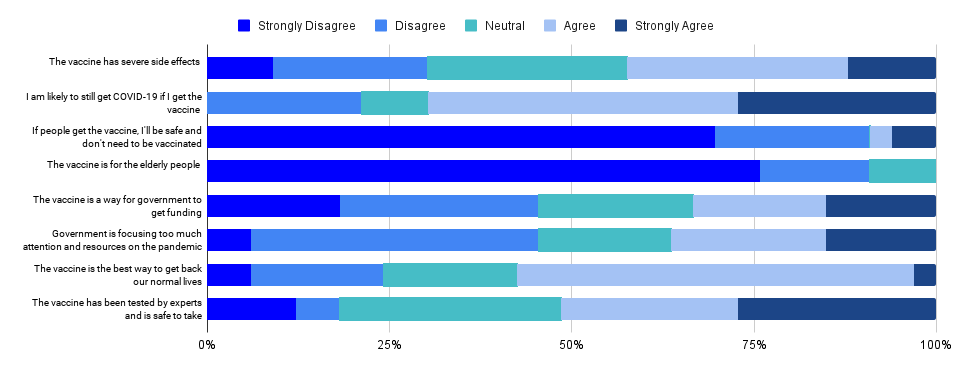
\includegraphics[width = \textwidth]{../../tables-figures/qual-beliefsKY.png} 
  \label{fig:qualKY}
\end{subfigure}
\begin{subfigure}{\textwidth}
  \centering
  \caption{Nigeria ($n = 40$)}
  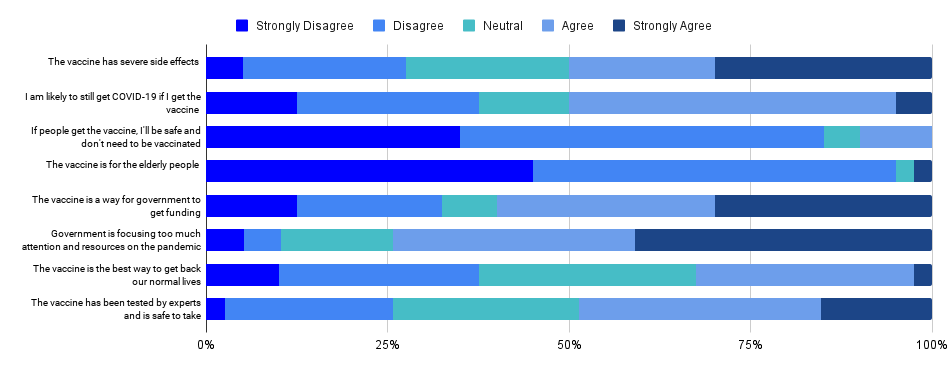
\includegraphics[width = \textwidth]{../../tables-figures/qual-beliefsNG.png} 
  \label{fig:qualNG}
\end{subfigure}
   \caption{Beliefs about the COVID-19 vaccine, based on focus group discussions conducted by the Busara Center for Behavioral Economics}
   \label{fig:qual}
\end{figure}


\subsubsection{Facebook pretest}
We collected data from a short, open-response survey on Facebook among respondents in Kenya and Nigeria. 320 respondents answered our short pretest survey, 89\% of whom live in Nigeria. 51\% of respondents reported they were not yet vaccinated against COVID-19. Of the respondents who reported being vaccinated, 60\% reported that they did not experience any side effects after getting the vaccine.

When we asked respondents who said they had gotten the vaccine why they chose to do so, several said it was because they wanted to protect themselves against COVID-19. A few indicated social reasons--either because they wanted to show/influence others, or because others had influenced them.

Many respondents said they were not vaccinated on account of the unavailability of the vaccine. Some said they weren't sure where to get the vaccine or referenced the need for money to get it. Others reported not having enough information about the vaccine and being afraid to get it.

One of the main goals of the pretest was to collect answers to the question:  ``What would you say is your main question or concern about the COVID-19 vaccine?'' Here we saw concern over side effects, questions about the vaccine's safety and effectiveness, and belief that the vaccine is not necessary because COVID-19 doesn't pose a serious threat.

\subsection{Quantitative study design}

The quantitative portion of the study occurs following the below stages: 

\begin{enumerate}
\item \textbf{Recruitment and pre-screening.} We have set up a Facebook page (\url{https://www.facebook.com/dataforsociety}) for the project, and will use Facebook advertisements to target and recruit social media users 18 years and older living in Kenya and Nigeria. Advertisements are targeted to achieve balance on gender, and over-sample respondents who are above national median ages (which are under-represented among social media users).\footnote{The median age of adults 18 years and older is 30 years in Nigeria \citep{afrobarometer-ng-2018} and 33 years in Kenya \citep{afrobarometer-ky-2020}.}

\begin{figure}[h!]
   \centering
   \begin{subfigure}{0.45\textwidth}
  \centering
  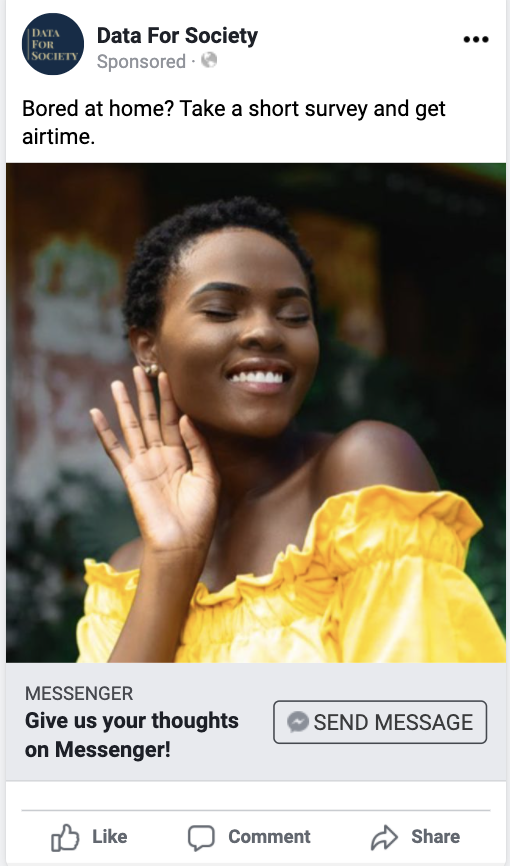
\includegraphics[width = \textwidth]{../../tables-figures/ad1.png} 
  \label{fig:ad1}
\end{subfigure}
\begin{subfigure}{0.45\textwidth}
  \centering
  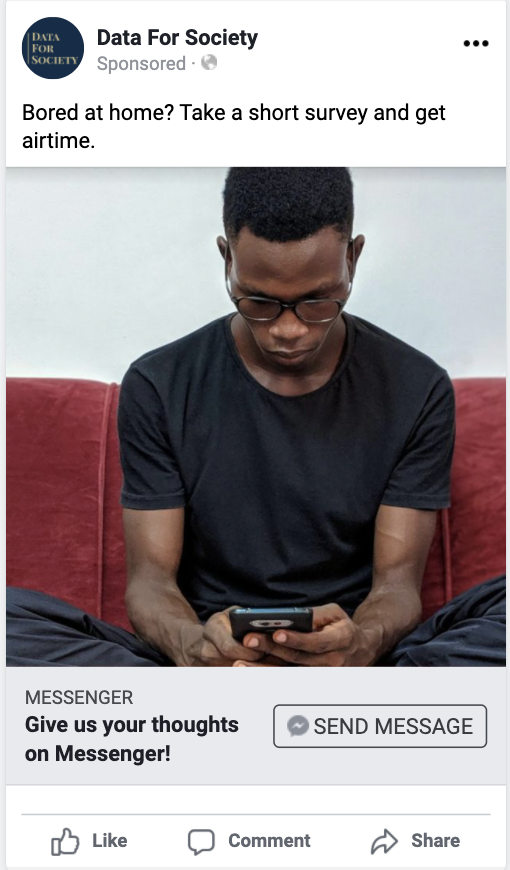
\includegraphics[width = \textwidth]{../../tables-figures/ad2.png} 
  \label{fig:ad2}
\end{subfigure}
   \caption{Facebook recruitment click-to-Messenger advertisements}
   \label{fig:ads}
\end{figure}

When respondents click to start a message on the advertisement, a Facebook Messenger conversation is started with our chatbot. All respondents, regardless of later treatment assignment, interact with the chatbot to take a survey. The initial conversation with the chatbot collects information on whether respondents have been vaccinated and tests whether respondents can view images on their Messenger app and are able to pass an attention check. 

\item \textbf{Select respondents.} We are interested in moving respondents who have not yet been vaccinated. Consequently, we then condition for continued engagement based on survey pre-screening responses: we continue with respondents who are vaccine ``unsure'' and report that they have not yet received any doses of a COVID-19 vaccine; we also ensure that respondents have passed pre-test checks. 

\item \textbf{Invitation to participate.} 24 hours after pre-screening, we invite eligible respondents to participate in the survey. After completing the full survey they receive the equivalent of USD 0.75 in mobile airtime. The 24 hour delay introduces a time buffer allowing us to further screen for any repeat survey takers who have created fake Facebook accounts. Based on prior experience with these surveys the hope is also to deter serial survey takers from repeatedly taking the survey since they may not know what qualifies for the invitation to participate in the full survey and because they need to wait in order to access. 

\item \textbf{Main survey.} We collect survey responses and deliver treatment using the chatbot. 

\item \textbf{Follow-up survey.} Three weeks after the survey, we use sponsored messaging advertisements to offer incentives of the equivalent of USD 0.25 in mobile airtime to participate in a short follow-up survey. The purpose of the follow-up survey is to measure effects on self-reported vaccination, providing respondents sufficient time after the delivery of the intervention to get vaccinated, if they wished.

\end{enumerate}

\begin{figure}[h!]
   \centering
   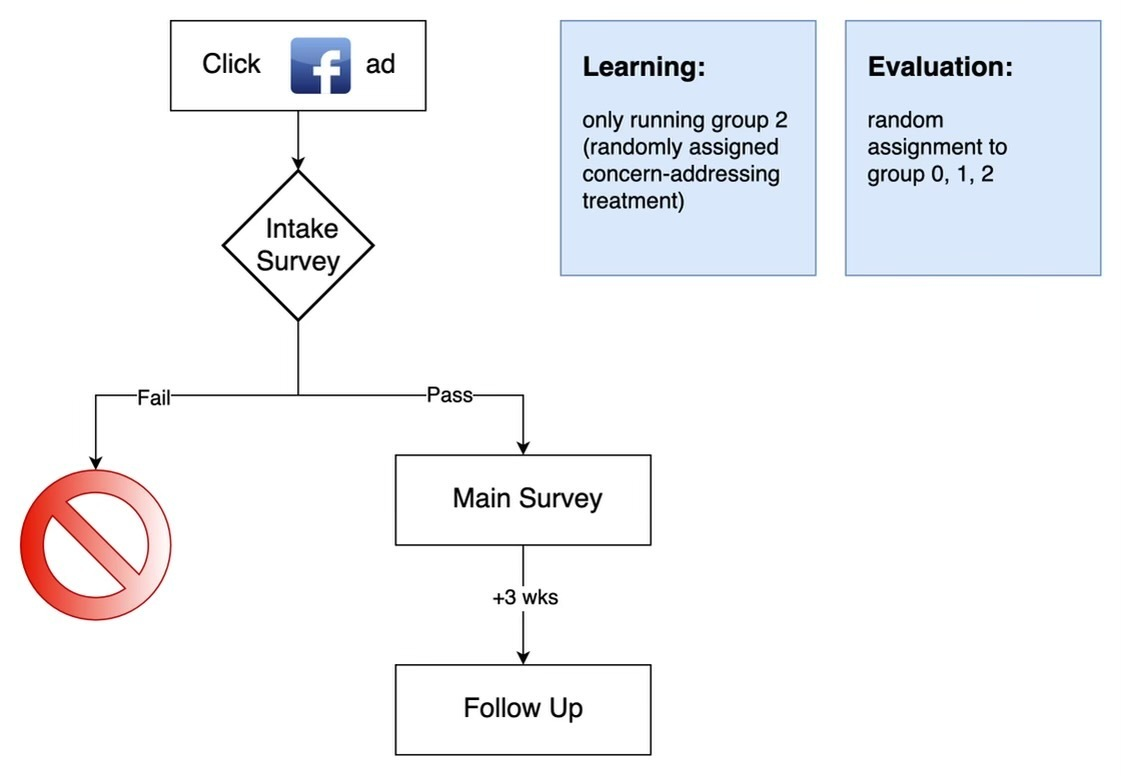
\includegraphics[width = 0.9\textwidth]{../../tables-figures/vcf_survey_flow.jpg} 
   \caption{Survey flow diagram.}
   \label{fig:surveyflow}
\end{figure}


\subsubsection{Messaging}

In the chatbot condition, we deliver targeted messaging based on what respondents report as their top concerns related to the vaccine. The response options were designed based on the pre-test survey that asked the same (open-ended) question and focus group discussions in both countries conducted by the Busara Center for Behavioral Economics. 

Respondents will be asked the following question with 8 possible answer options:\footnote{The ``other'' option will be included in the learning phase only. }

\begin{table}[htbp]
   \centering
\begin{tabular}{p{.3\textwidth}  l}
  & \multicolumn{1}{c}{ \textit{Order randomized at the respondent level} } \\
  \raggedright
What would you say is your main question or concern about the COVID-19 vaccine? & 
\begin{tabular}{p{.6\textwidth}} 
\hline
\begin{enumerate}[itemsep = -0.9ex, topsep = 0ex, partopsep=0ex, parsep=1ex, leftmargin=2ex, labelindent=\parindent]
\item I'm worried about the side effects of the vaccine.
\item I don't know if the vaccine works.
\item I don't think COVID-19 is real.
\item I don't need the vaccine because I am protected by God.
\item I don't trust healthcare workers.
\item I don't trust the government.
\item I am hearing different things about the vaccine, and I'm not sure what to believe is true and what is false.
\item Other (specify). 
\end{enumerate}
\end{tabular}
\end{tabular}
   \caption{Concern elicitation and categorization.}
   \label{tab:concerns}
\end{table}


Table \ref{tab:mapping} illustrates how the messages map onto the different main concerns. After providing the messaging associated with a given concern, we then ask respondents if they have any additional concerns. If they have additional concerns, they may continue engaging with chatbot and receiving targeted messaging related to each subsequent concern. They may engage with the chatbot for up to three concerns. 


\begin{table}[htbp]
   \centering
   \begin{tabular}{@{\extracolsep{4pt}}p{.5\textwidth}  l}
\multicolumn{1}{c}{ \textbf{Concern} } & \multicolumn{1}{c}{ \textbf{Messages} } \\
\cline{1-1}  \cline{2-2}
1. I'm worried about the side effects of the vaccine. & 
\begin{tabular}{p{.4\textwidth}} 
\begin{itemize}[itemsep = -0.9ex, topsep = 0ex, partopsep=0ex, parsep=1ex, leftmargin=2ex, labelindent=\parindent, nosep]
\item Vaccine side effects (mild) 
\item Vaccine side effects (debunk) 
\item Benefits 
\item Risks \vspace*{-\baselineskip}
\end{itemize}
\end{tabular} \\
2. I don't know if the vaccine works.& 
\begin{tabular}{p{.4\textwidth}} 
\begin{itemize}[itemsep = -0.9ex, topsep = 0ex, partopsep=0ex, parsep=1ex, leftmargin=2ex, labelindent=\parindent]
\item How vaccines work 
\item Misinfo (AfricaCheck video)
\item elite cues (WHO)
\item elite cutes (political leaders) \vspace*{-\baselineskip}
\end{itemize}
   \end{tabular}
\\
3. I don't think COVID-19 is real.& 
\begin{tabular}{p{.4\textwidth}} 
\begin{itemize}[itemsep = -0.9ex, topsep = 0ex, partopsep=0ex, parsep=1ex, leftmargin=2ex, labelindent=\parindent]
\item Benefits
\item Elite cues (religious leaders) 
\item Misinfo (accuracy prime)
\item Misinfo (AfricaCheck video) \vspace*{-\baselineskip}
\end{itemize}\end{tabular}
\\
4. I don't need the vaccine because I am protected by God.& 
\begin{tabular}{p{.4\textwidth}} 
\begin{itemize}[itemsep = -0.9ex, topsep = 0ex, partopsep=0ex, parsep=1ex, leftmargin=2ex, labelindent=\parindent]
\item Benefits 
\item  Social considerations 
\item  Elite cues (religious leaders)\vspace*{-\baselineskip}
\end{itemize}\end{tabular}
\\
5. I don't trust healthcare workers.& 
\begin{tabular}{p{.4\textwidth}} 
\begin{itemize}[itemsep = -0.9ex, topsep = 0ex, partopsep=0ex, parsep=1ex, leftmargin=2ex, labelindent=\parindent]
\item Elite cues (political) 
\item  Elite cues (WHO) 
\item  Elite cues (religious leaders) 
\item  Vaccine development/approvals
\item  Vaccine safety/effectiveness  \vspace*{-\baselineskip}
\end{itemize}\end{tabular}
\\
6. I don't trust the government.& 
\begin{tabular}{p{.4\textwidth}} 
\begin{itemize}[itemsep = -0.9ex, topsep = 0ex, partopsep=0ex, parsep=1ex, leftmargin=2ex, labelindent=\parindent]
\item Elite cues (WHO)
\item Elite cues (healthcare) 
\item Elite cues (religious leaders) 
\item Vaccine development/approvals 
\item Vaccine safety/effectiveness \vspace*{-\baselineskip}
\end{itemize}\end{tabular}
\\
7. I am hearing different things about the vaccine, and I'm not sure what to believe.& 
\begin{tabular}{p{.4\textwidth}} 
\begin{itemize}[itemsep = -0.9ex, topsep = 0ex, partopsep=0ex, parsep=1ex, leftmargin=2ex, labelindent=\parindent]
\item Misinfo (Facebook tips) 
\item Misinfo (AfricaCheck video) 
\item Misinfo (accuracy prime)
\item Misinfo (7 types) 
\item Vaccine side effects (debunk) \vspace*{-\baselineskip}
\end{itemize}
   \end{tabular}
\\   
   8. Other (specify).& 
\begin{tabular}{p{.4\textwidth}} 
\begin{itemize}[itemsep = -0.9ex, topsep = 0ex, partopsep=0ex, parsep=1ex, leftmargin=2ex, labelindent=\parindent]
\item PSA message
\end{itemize}
   \end{tabular}
   \end{tabular}
   \caption{Mapping messages to stated concerns.}
   \label{tab:mapping}
\end{table}

After respondents report their primary concern, we deliver messaging targeted to that concern. In the learning phase messaging is assigned randomly within the set of messages targeting that particular concern, as outlined in Table~\ref{tab:mapping}. In the evaluation phase, the top performing message(s) in each category will be assigned for each concern. (See Section ~\ref{message} for further discussion of messaging selection.)

\clearpage
The content of the messages is as follows:

\begin{enumerate}
  \item \textbf{Vaccine side effects (mild)} emphasizes that most side effects are mild, short-lived, and some people experience no side effects to the vaccine. 
  \item \textbf{Vaccine side effects (debunk)} corrects common misperceptions about COVID-19 vaccine side effects, particularly that the vaccine does not make you magnetic and that it is safe (and encouraged) for pregnant women. We also share a link debunking other common rumors from AfricaCheck.org.
  \item \textbf{Vaccine development/approvals} describes how the road to develop the COVID-19 vaccine had several checkpoints where experts (both national and international bodies) verified the safety of the vaccine, and provides links to short videos from the AfricaCheck.org on how vaccines are vetted and how COVID-19 vaccines were created so quickly. 
  \item \textbf{Vaccine safety/effectiveness} describes what it means when people say vaccines are safe and effective and presents information from the WHO related to COVID-19 vaccine safety.
  \item \textbf{Benefits} makes salient the myriad benefits to vaccination, particularly focusing on ``getting back to normal life'' since many faced economic hardships from lockdowns and the impacts of the global pandemic this message appeals to those interests and emotions and suggests vaccination may be the fastest way back to normal. We also randomize within this message to test whether priming respondents that government services may be contingent upon being vaccinated against COVID-19 in the future.
  \item \textbf{Risks} describes the risks associated with COVID-19 and how the likelihood of severe illness and death from the virus is much lower among vaccinated individuals.
  \item \textbf{How vaccines work} provides a \href{https://www.facebook.com/dataforsociety/videos/4265014093602814}{link} to a video explaining how the COVID-19 vaccine helps to prevent the disease in the body. 
  \item \textbf{Social considerations} informs respondents that a vaccine not only protects an individual, but also others around them, and includes a video explaining herd immunity. It asks respondents to not only consider themselves but also others who might be vulnerable to the virus but who cannot receive themselves and would benefit from as many people as possible getting vaccinated.
  \item \textbf{Elite cues posts} presents images and videos from different types of elites getting the COVID-19 vaccine themselves and endorsing it. 
  \begin{enumerate}[noitemsep, topsep=0pt]
    \item \textbf{Political figures}: photo of the president of the country receiving the COVID-19 vaccine
    \item \textbf{International experts}: photo of Dr. Tedros Adhanom Ghebreyesus, Director General of the World Health Organization (WHO) receiving his COVID-19 vaccine.
    \item \textbf{Religious figures}: muslim and christian leaders endorsing COVID-19 vaccination.
    \item \textbf{Healthcare workers}: videos of healthcare workers in each country endorsing vaccination.
  \end{enumerate}
  \item \textbf{Misinformation}
    \begin{enumerate}[noitemsep, topsep=0pt]
    \item \textbf{Facebook tips} presents 5 tips Facebook suggests to help spot misinformation (generally).
    \item \textbf{AfricaCheck video} presents 5 general tips to help spot misinformation, generally. And also presents a video for suggestions on how to identify COVID-19 misinformation.
    \item \textbf{Pledge} adapted from \cite{offer-westort2021optimal}. it asks people to take a pledge (and post to their timeline if they choose to) to spot and speak out about misinformation to help keep friends and family safe from COVID-19 misinformation.\footnote{The pledge is only assigned as a secondary treatment, in addition the Facebook tips treatment, the AfricaCheck video, or the accuracy prime. }
    \item \textbf{Accuracy} prime is based on an accuracy nudge that has been proven effective in this and other contexts \citep{pennycook2020fighting, offer-westort2021optimal}, but rather than asking people to think about whether an actual post (stimuli) is true or not, we prime respondents to think about accuracy, generally, when they're scrolling through social media.
    \item \textbf{7 types of misinformation} teaches respondents the different types of misinformation they may encounter (e.g, misleading content, fake experts, satire, etc.) as categorized by \href{https://firstdraftnews.org/}{First Draft}, and then asks respondents to take a quiz and test whether they can correctly identify the type of misinformation on a false COVID-19 vaccine post. 
  \end{enumerate}
  \item {Public service messaging} delivers a generic message encouraging vaccine uptake. 
  \begin{figure}[h!]
   \centering
   
\includegraphics[width = 0.45\textwidth]{../../tables-figures/psa.png} 
   \caption{Public service messaging.}
   \label{fig:psa}
\end{figure}
\end{enumerate}


\subsubsection{Outcome measurement}

\paragraph{Primary outcome}
Our primary outcome is self-reported willingness and intention to get the COVID-19 vaccine.

We ask the following questions as measures of vaccine acceptance and intention to get vaccinated. 

\begin{itemize}
\item ``How much do you want to get a COVID-19 vaccine?''
\begin{itemize}[noitemsep, topsep=0pt]
\item Not at all (1)
\item A little (2)
\item Moderately (3)
 \item Very much (4)
\end{itemize}
\item ``If a COVID-19 vaccine were offered to you today (free of charge), would you choose to get vaccinated?''
\begin{itemize}[noitemsep, topsep=0pt]
\item No, definitely not (1) 
\item No, probably not (2)
\item Yes, probably (3)
\item Yes, definitely (4)
\end{itemize}
\end{itemize}

We standardize responses for each question separately and then add individual scores for a combined measure. 

\paragraph{Secondary outcome}
\begin{itemize}
\item \textbf{Sharing.} Following the primary outcome measurement, we also measure respondent sharing intentions with respect to both false and true social media posts about COVID-19 vaccines. After we show respondents each post, we ask them 
\begin{itemize}[noitemsep, topsep=0pt]
  \item ``Would you like to share this post on your timeline?''
  \item ``Would you like to send this post to a friend on Messenger?''
\end{itemize}
We report results with respect to sharing intentions for true and false posts separately. We expect that the extent to which sharing behavior is moved by messaging will be a consequence of the proportion of respondents who report uncertainty over information (concern seven) as their primary concern. 
\item \textbf{Information seeking.} As an interim behavioral measure we are also interested in whether respondents click on links advertising more information about the COVID-19 vaccine and, when available, links to registration sites to sign up for an appointment. The outcome variable is a binary variable for whether respondents clicked the link. 
\item \textbf{Encouraging others.} We also measure whether respondents share to their Facebook timeline a pro-vaccine post that we provide them with. The outcome variable is a binary variable for whether respondents clicked the link to share the post. 
\item \textbf{Vaccination status.} In the follow-up survey, we measure whether respondents have reported that they have received at least one dose of the vaccine. The outcome variable is a binary variable for whether respondents report that they have received at least one dose of the vaccine. 
\end{itemize}

\section{Learning and Evaluation}

\subsection{Learning phase}

The first 2,000 respondents in each country participate in the learning phase. In the learning phase, we will learn which messages are most effective in response to respondent concerns.  For example, respondents who articulate that they don't need the vaccine because they are protected by God (concern four) will be assigned the \textit{benefits}, \emph{social considerations}, or \emph{elite cues (religious leaders)} message. During the learning phase we learn which of these three messages is most effective for respondents who share this main concern. For this reason, in the learning phase, we assign all respondents to the group 2, condition: Chatbot, conditional vaccine interventions. 

We use data only from the first three concerns that respondents report.\footnote{We allow respondents to potentially receive the same message multiple times based on the concerns they articulate and the randomly assigned messaging.} We allow respondents to engage with the chatbot and submit multiple concerns, as there may be multiple topics contributing to individual vaccination decisions, and we believe that we can learn from individuals about messaging across these topics. However, as respondents engage with the chatbot for longer, the effects of individual messaging may diminish relative to the cumulative effects of past messages. 

After we deliver messaging related to the concern, we ask whether the messaging addressed their concern. A message is coded as a success only if the respondent responds affirmatively to this question. We use this direct measure of message efficacy rather than the eventual outcome of vaccine acceptance intentions, to get a less noisy measure to input into our adaptive algorithm. This also allows us to collect multiple measures per individual. 

\subsubsection{Adaptive algorithms}
We use a data-driven approach to learning, using an adaptive algorithm. We use a top-two Thompson sampling algorithm \citep{russo16a}, which assigns treatment with equal probability to the two treatment arms with the highest sampled posterior values. Our adaptive algorithm operates separately for each concern category, where ``treatments'' are the associated messages listed in Table~\ref{tab:mapping}. While the same message may be used in response to multiple concern categories, information about message efficacy is not shared across concern categories.  

For the first batch of 100 observations in each concern category, we assign treatment uniformly at random, to decrease algorithm instability from random noise early on in data collection; this batch is parameterized by gamma in the algorithm below. We also augment the top-two Thompson sampling algorithm to include probability floors, so that all arms are sampled with some minimal probability for every observation. In the description of the algorithm below, floors are set by the $\delta$ parameter; we set $\delta$ = 0.1, so that in each category, arms are sampled with a probability floor of $0.1 \times$ number of treatment arms in the concern category. So, for example, if there are three treatment messages that could be sent for a given concern, the floor is $0.1\times0.33 = 0.033$ for any given arm. After imposing floors, the remaining assignment probability is equally divided between the top two arms. The top two arms would be assigned treatment with probability 0.467, and the remaining arm is assigned treatment with probability 0.033.

We use the binary success measure described above as our reward for optimization. 


%In the learning phase, we will learn which messages are most effective in response to respondent concerns.  Consequently in the learning phase, we assign all respondents to the group 2, condition: Chatbot, conditional vaccine interventions.
%
%We use data only from the first three concerns that respondents report. After we deliver messaging related to the concern, we ask whether the messaging addressed their concern, with the options: yes, not really. Values are assigned as (1, 0) respectively, i.e., the message is a success only if it addresses the question. At the end of the learning phase, we select messaging based on messages with the highest inverse probability weighted average value for each concern category. 
%
%In this stage, we assign treatment using top-two Thompson sampling \cite{russo16a} within each concern category, with a probability floor of 0.1/|category|.

We suppose that $K$ arms have unknown success rates $\theta_1, \dots, \theta_K$, following their respective Bernoulli distributions, with likelihoods
\[f_{X_1|\Theta_1}(x_1|\theta_1),\dots, f_{X_K|\Theta_K}(x_K|\theta_K).\]
Posteriors follow Beta distributions with parameters $\alpha_{k,b}, \beta_{k,b}$. 

The design below is parameterized by our priors, set as uniform for all arms, $\alpha_{k} = \beta_{k} =1$; a value $\gamma$ which sets the first batch size for uniform random assignment; and a value $\delta$, which sets the probability floor. 

\begin{algorithm} \footnotesize
    \caption{Top-two Thompson sampling with probability floors}
    \label{algg:ttts}
    \begin{algorithmic}[1] % The number tells where the line numbering should start
    	\State Set  $\alpha_{k} \leftarrow 1, \ \beta_{k} \leftarrow 1\ \forall k \in \kk$%; \aB \leftarrow \y \leftarrow $ empty vector.  
	\Comment{Initialize priors}%, assignment vector, and reward vector. }
    	\For{$i = 1, \dots, N$}
		\If{$i \leq \gamma$}
			 \State Set $p_{k} \leftarrow \frac{1 }{|\kk| } \ \ \forall k \in \kk $ \Comment{In first batch, set treatment probabilities as uniform.}
		\Else 	
			\For{$k \in \kk$}
				\State Sample $\hat \theta_k  \sim \textrm{Beta}\left(\alpha_{k}, \beta_{k} \right)$ \Comment{Sample from posteriors. }
			 \EndFor
			\State Set $I_1 \leftarrow \underset{k}{\argmax} \hat\theta_k$; set $I_2 \leftarrow \underset{j\neq I_1}{\argmax} \hat\theta_j$. \Comment{Identify top two arms from posterior samples}. 
			\State Set $p_k \leftarrow {\delta \times |\kk| } $ for $k \notin \{ I_1, I_2\} $. \Comment{Assign probabilities floors for not top two arms.}
			\State Set $p_k \leftarrow \frac{1}{2} (1-  \sum\limits_{j \notin \{ I_1, I_2\} } p_j) $ for $k \in \{ I_1, I_2\} $ \Comment{Assign remaining probability equally to top two arms.}
		\EndIf
		\State Assign treatment $a_i$ with probabilities $\p = \{ p_k: k \in \kk \} $; observe rewards $y_i$.
%		\State $\aB \leftarrow [\aB : a_i]$ \Comment{Augment assignment vector.}
%		\State $\y \leftarrow [\y : y_i]$ \Comment{Augment reward vector vector.}
		\For{$k \in \kk$} \Comment{Update posterior distribution parameters.}
			\State $(\alpha_{k}, \beta_{k}) \leftarrow (\alpha_{k} + \mathbbm{1}\{ a_i = k\}\mathbbm{1}\{ y_i = 1\} + 1,  \beta_{k} + \mathbbm{1} \{ a_i = k\}\mathbbm{1}\{ y_i = 0\})$. 
		\EndFor	
	\EndFor
    \end{algorithmic}
\end{algorithm}

\begin{figure}[htbp]
   \centering
   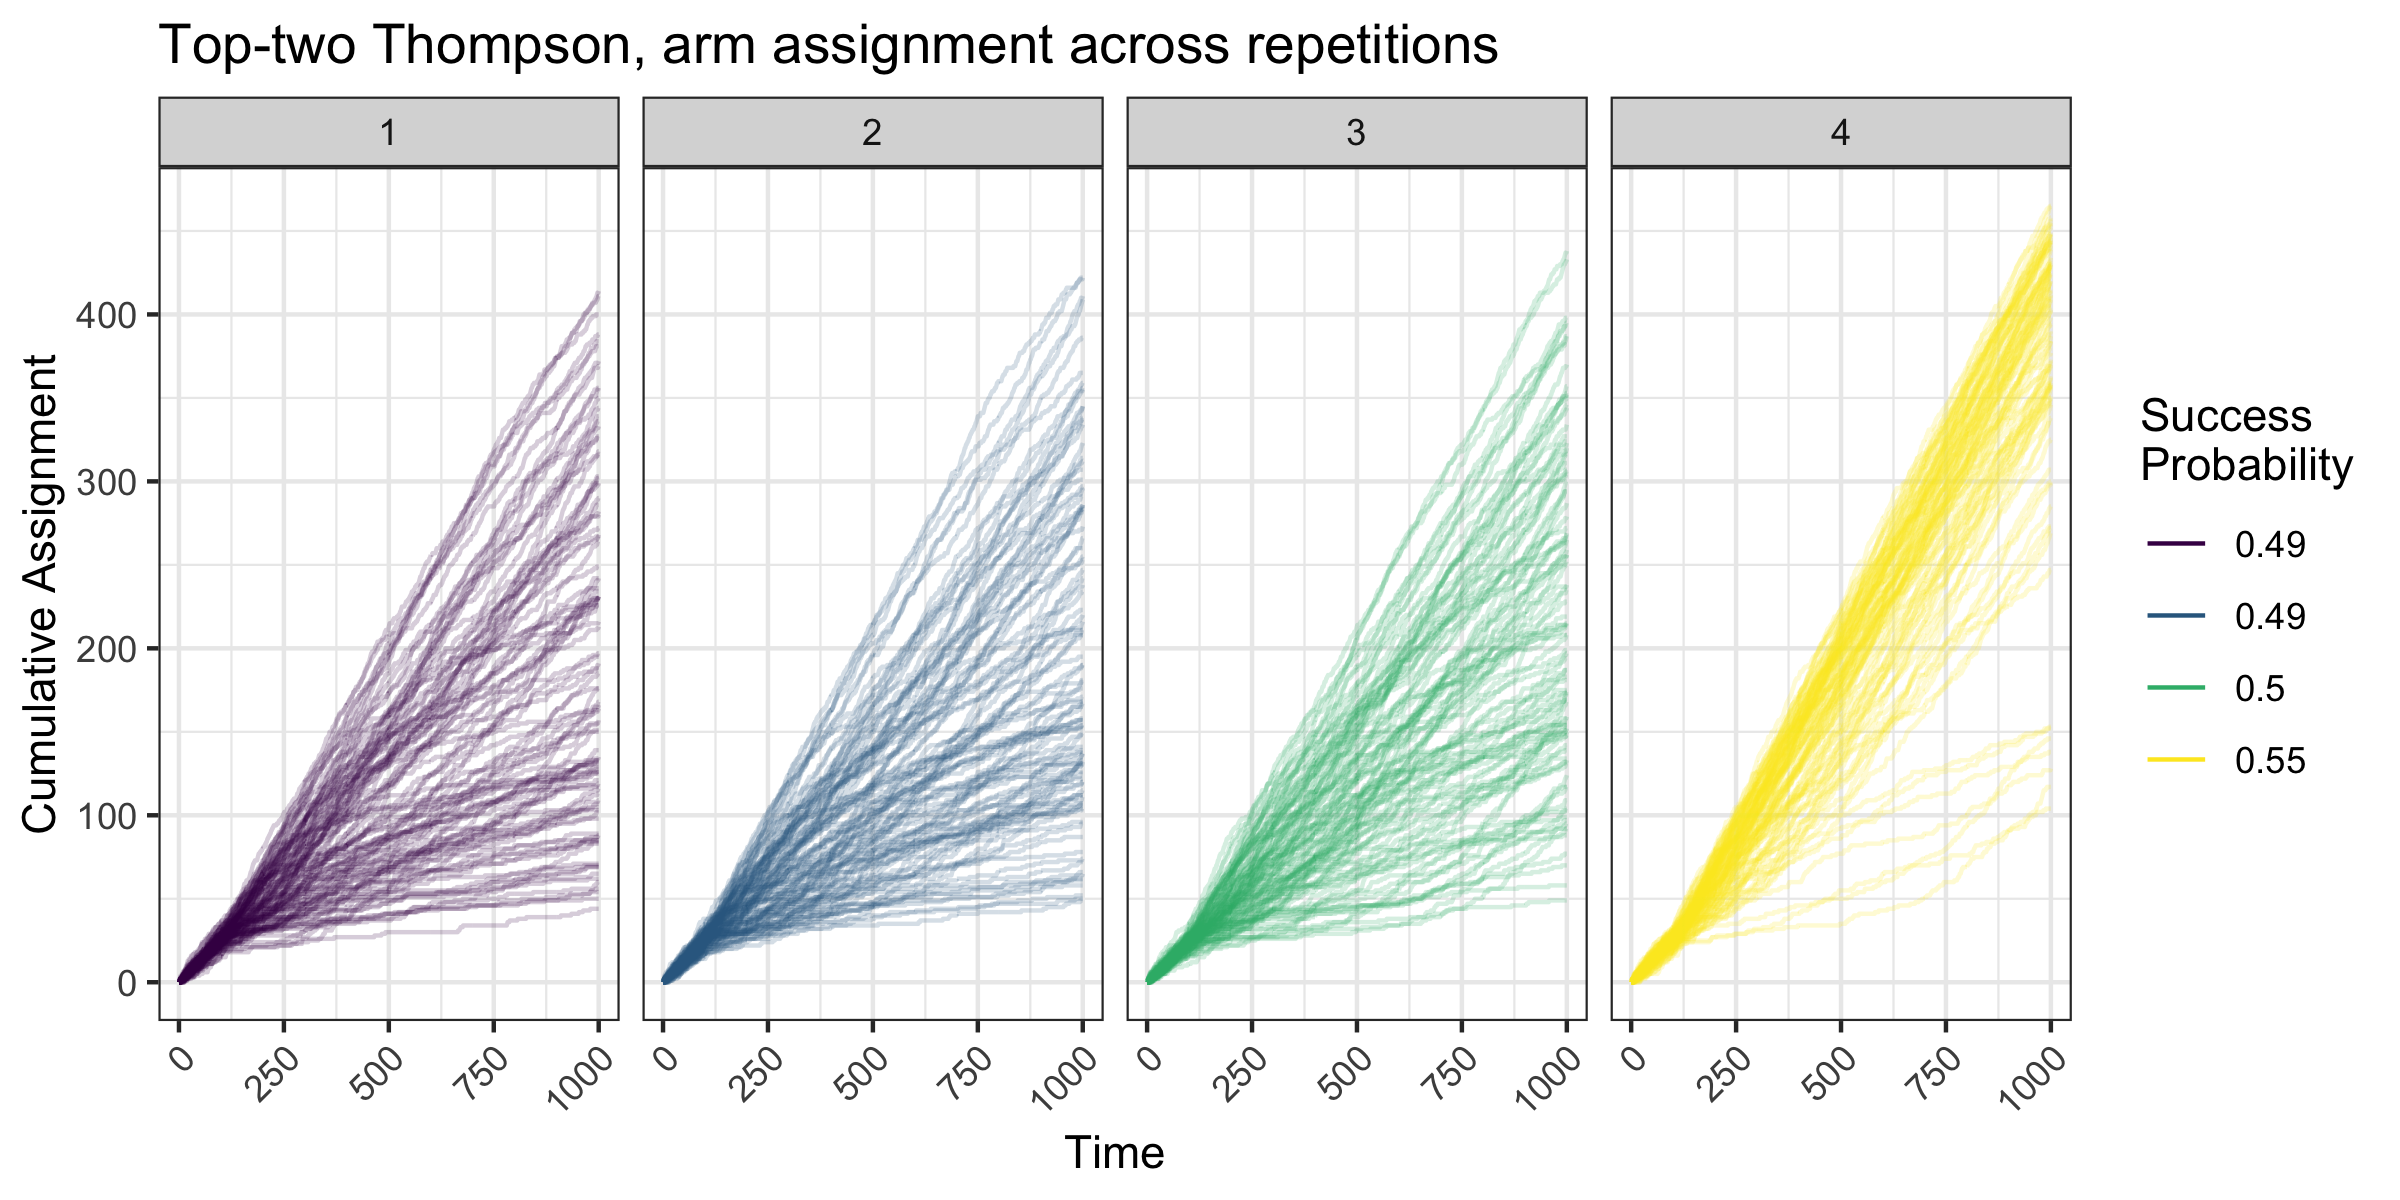
\includegraphics[width = 0.95\textwidth]{../../tables-figures/tt_cumulative4.png}
   \caption{Top-two Thompson sampling, arm assignment across repetitions. Using four arms and success probabilities 0.49, 0.49, 0.5, and 0.55, this figure shows cumulative assignment to each arm over repeated simulated experiments. }
   \label{fig:ttt_cumulative}
\end{figure}


\subsubsection{Message selection}\label{message}

At the end of the learning phase, we will determine which messaging treatments are most effective for each concern category using stabilized inverse probability weighted estimates of mean response rates. 

Figure~\ref{fig:ttt_best} shows the rate at which we select the best arm in a simulated experimental condition. With 2,000 observations per country, assuming each respondent reports 1.5 concerns, we will have on average 850 observations for each adaptive algorithm; our simulation shows that we will select the best arm 76\% of the time in this setting using the sample mean or stabilized inverse probability weights, when the best arm improves over the second best arm by 0.05 percentage points. We will select one of the two best arms 89\% of the time. 


\begin{figure}[htbp]
   \centering
   \begin{subfigure}{\textwidth}
  \centering
  \caption{Top arm selected}
  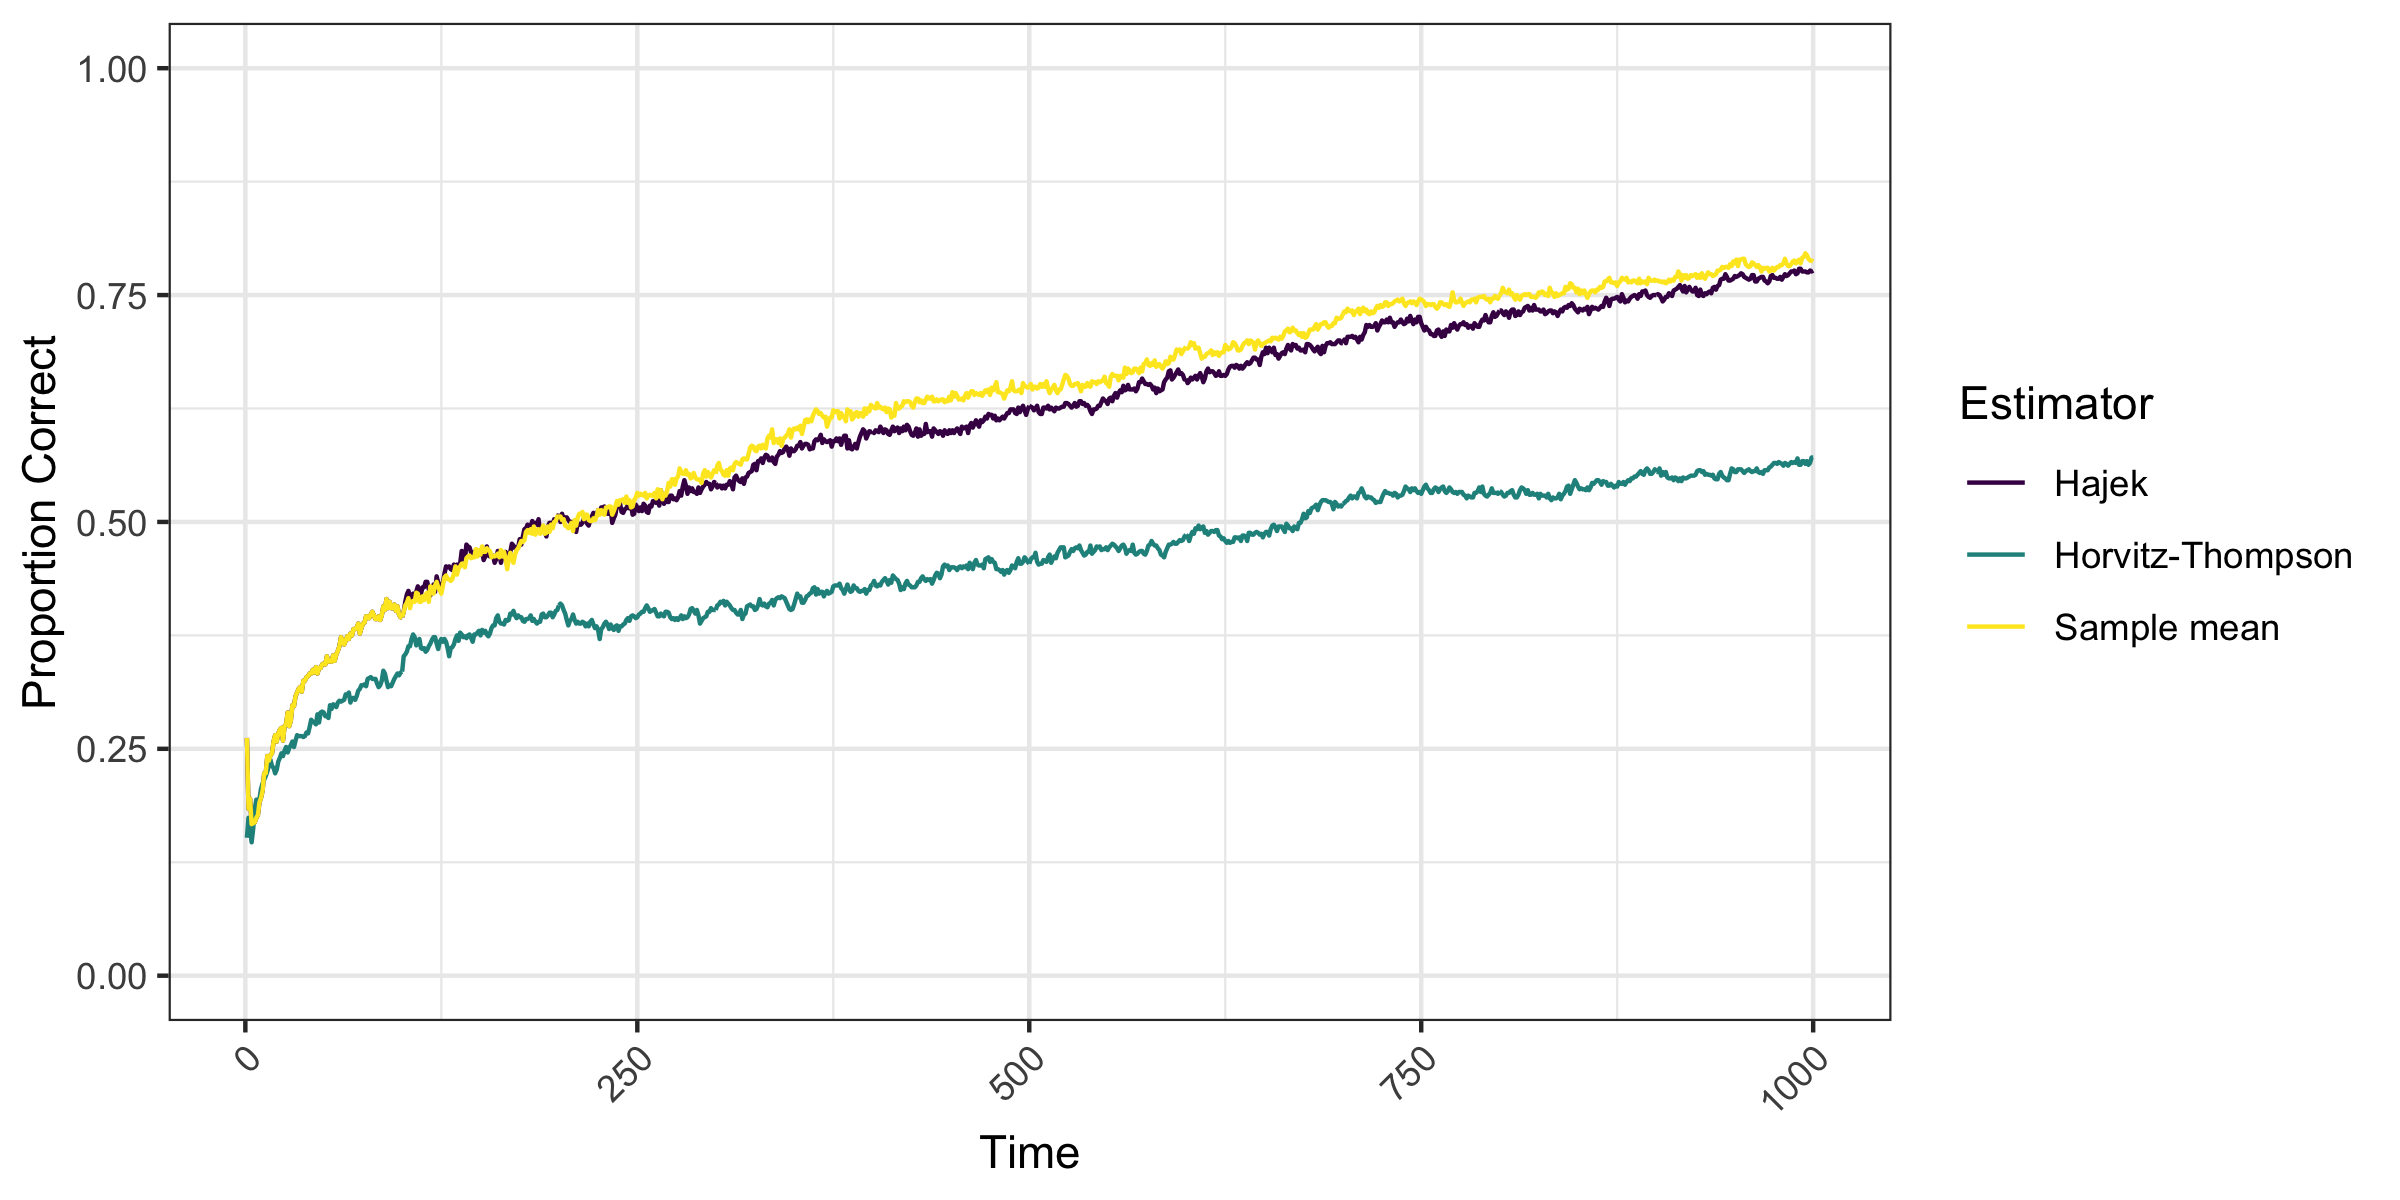
\includegraphics[width = \textwidth]{../../tables-figures/tt_correct4.png} 
  \label{fig:tt_best1}
\end{subfigure}
\begin{subfigure}{\textwidth}
  \centering
  \caption{One of top two arms selected}
  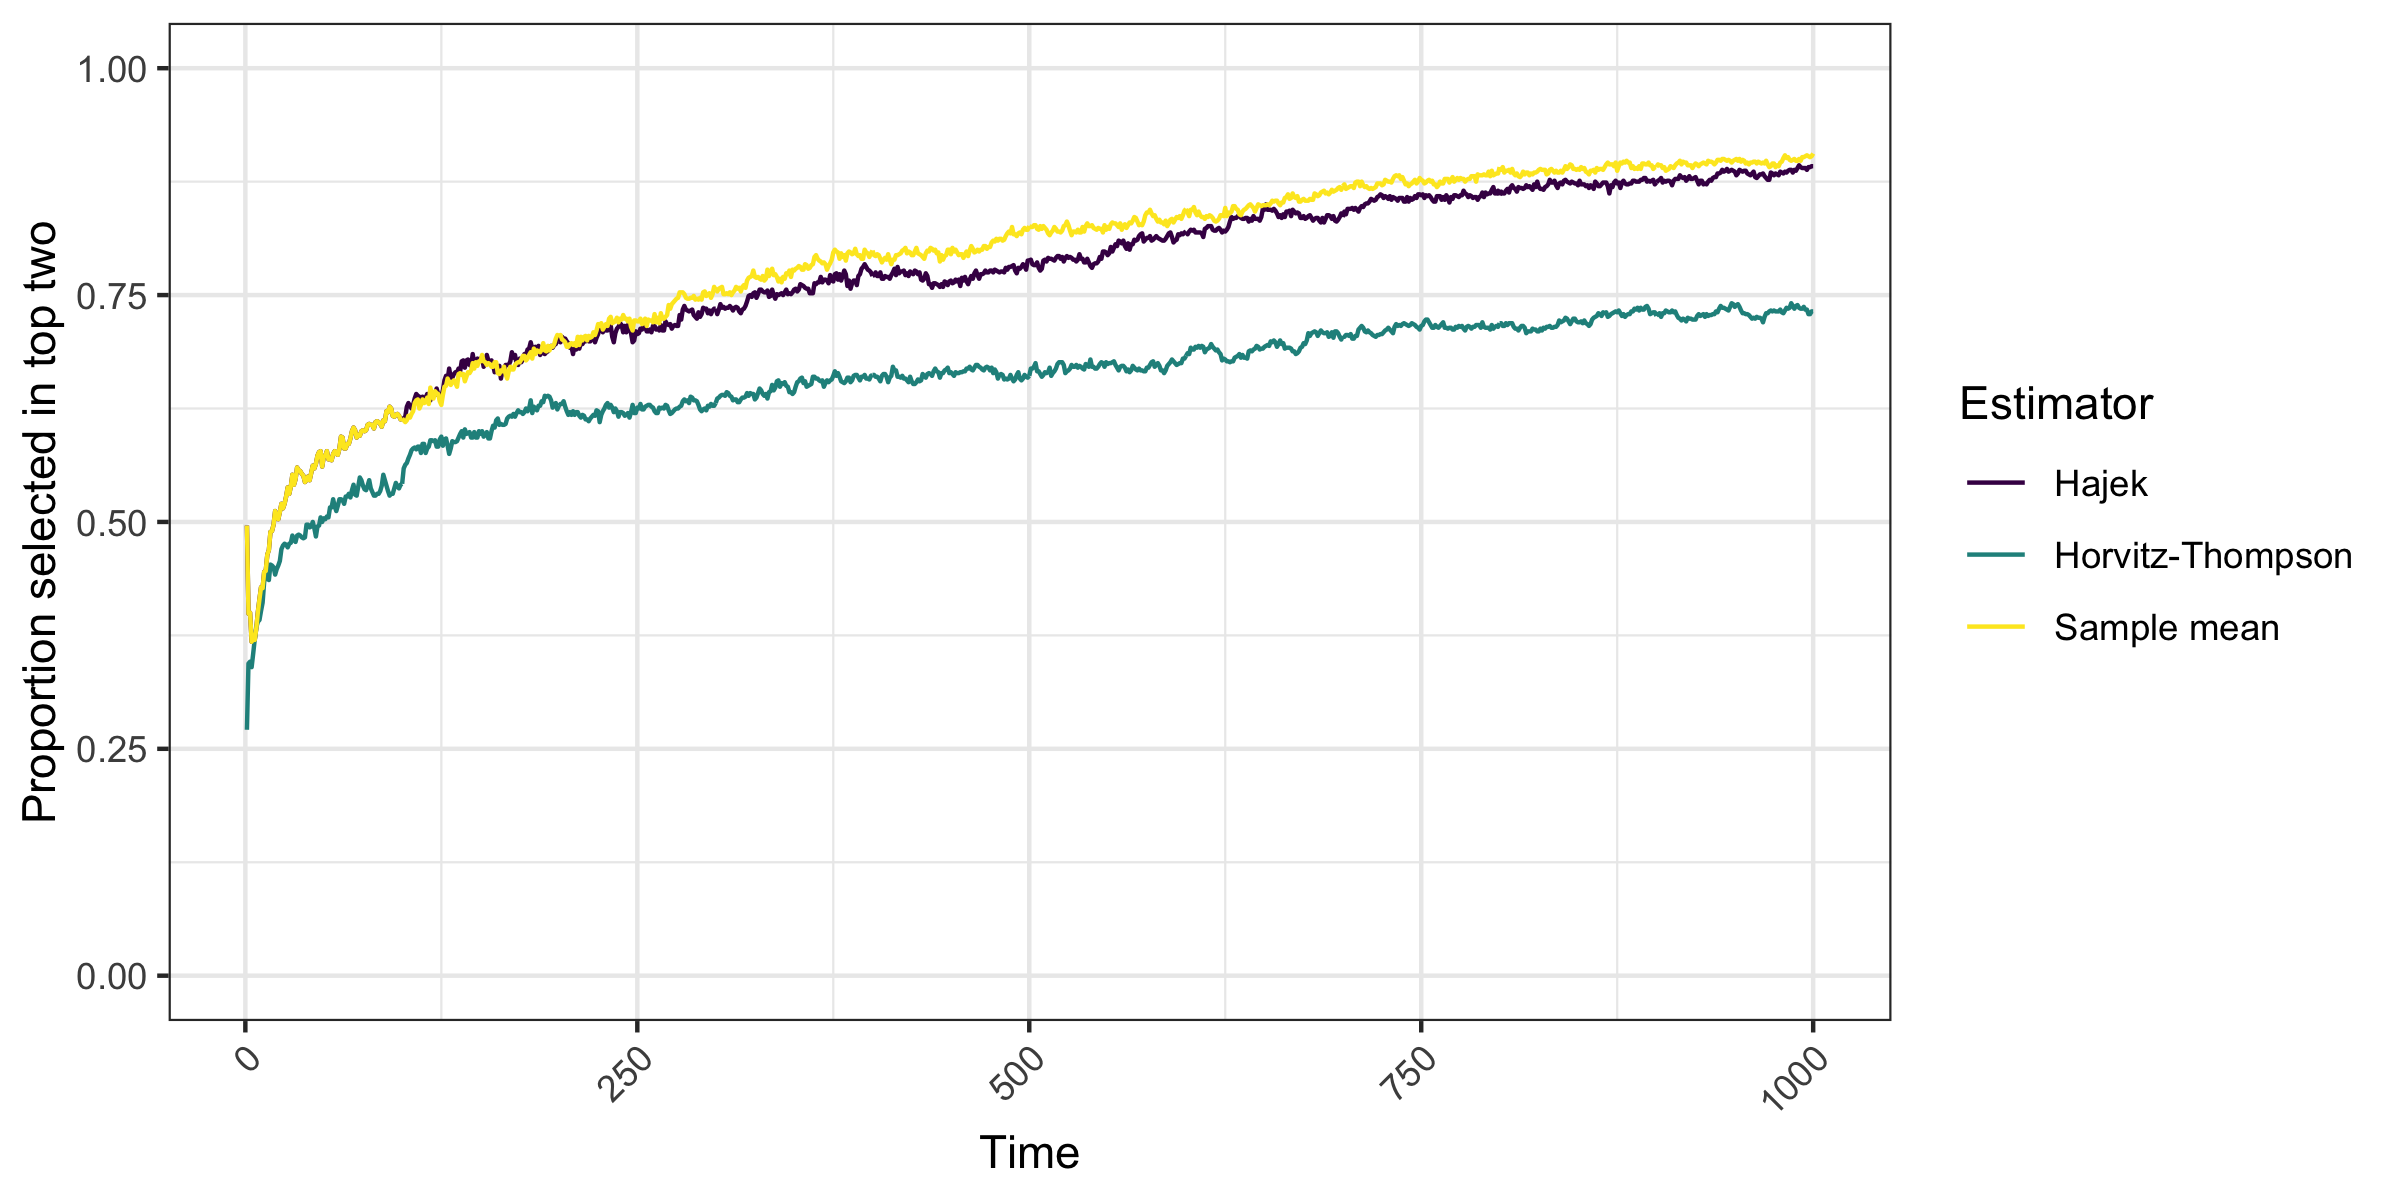
\includegraphics[width = \textwidth]{../../tables-figures/tt_correct-top-two4.png} 
  \label{fig:tt_best2}
\end{subfigure}
   \caption{Top-two Thompson sampling, best arm selection across repetitions. Using four arms and success probabilities 0.49, 0.49, 0.5, and 0.55, this figure represents the proportion of the times the true best arm (panel a), or one of the top two arms (panel b) is selected across 1,000 simulated experiments, using different estimators for arm selection.}
   \label{fig:ttt_best}
\end{figure}

We use stabilized inverse probability weights because they perform approximately as well as the sample mean in best arm selection, but they do not have the large bias problems of the sample mean. Estimates under the sample mean using adaptively collected data are systematically biased \citep{nie2017adaptively}.  Figure~\ref{fig:ttt_bias} shows the bias of each estimator for each arm in our simulated setting; as more data is collected for the best arm, bias is reduced, but for under-performing arms without sufficient probability floors, bias may persist asymptotically. We address this bias by using inverse probability weighted estimators. The Horvitz-Thompson estimator is finite-sample unbiased (see \citealt{bowden2017unbiased}; \citealt{offer2021adaptive} also shows a proof of this in Appendix B.2.). The stabilized inverse probability weighted estimator is approximately unbiased and has lower variance than the Horvitz-Thompson estimator--explaining the better performance in best arm selection in Figure~\ref{fig:ttt_best}. 

We will validate the message efficacy measure against vaccine intentions, checking that there is positive correlation. When the estimated response of the second best message is within 0.05 standard deviations of the best message, we will randomize across the best two messages. We will assign only these selected messages to respondents in conversation with the concern-responding chatbot based on the respondent-provided concern category. 


\begin{figure}[htbp]
   \centering
   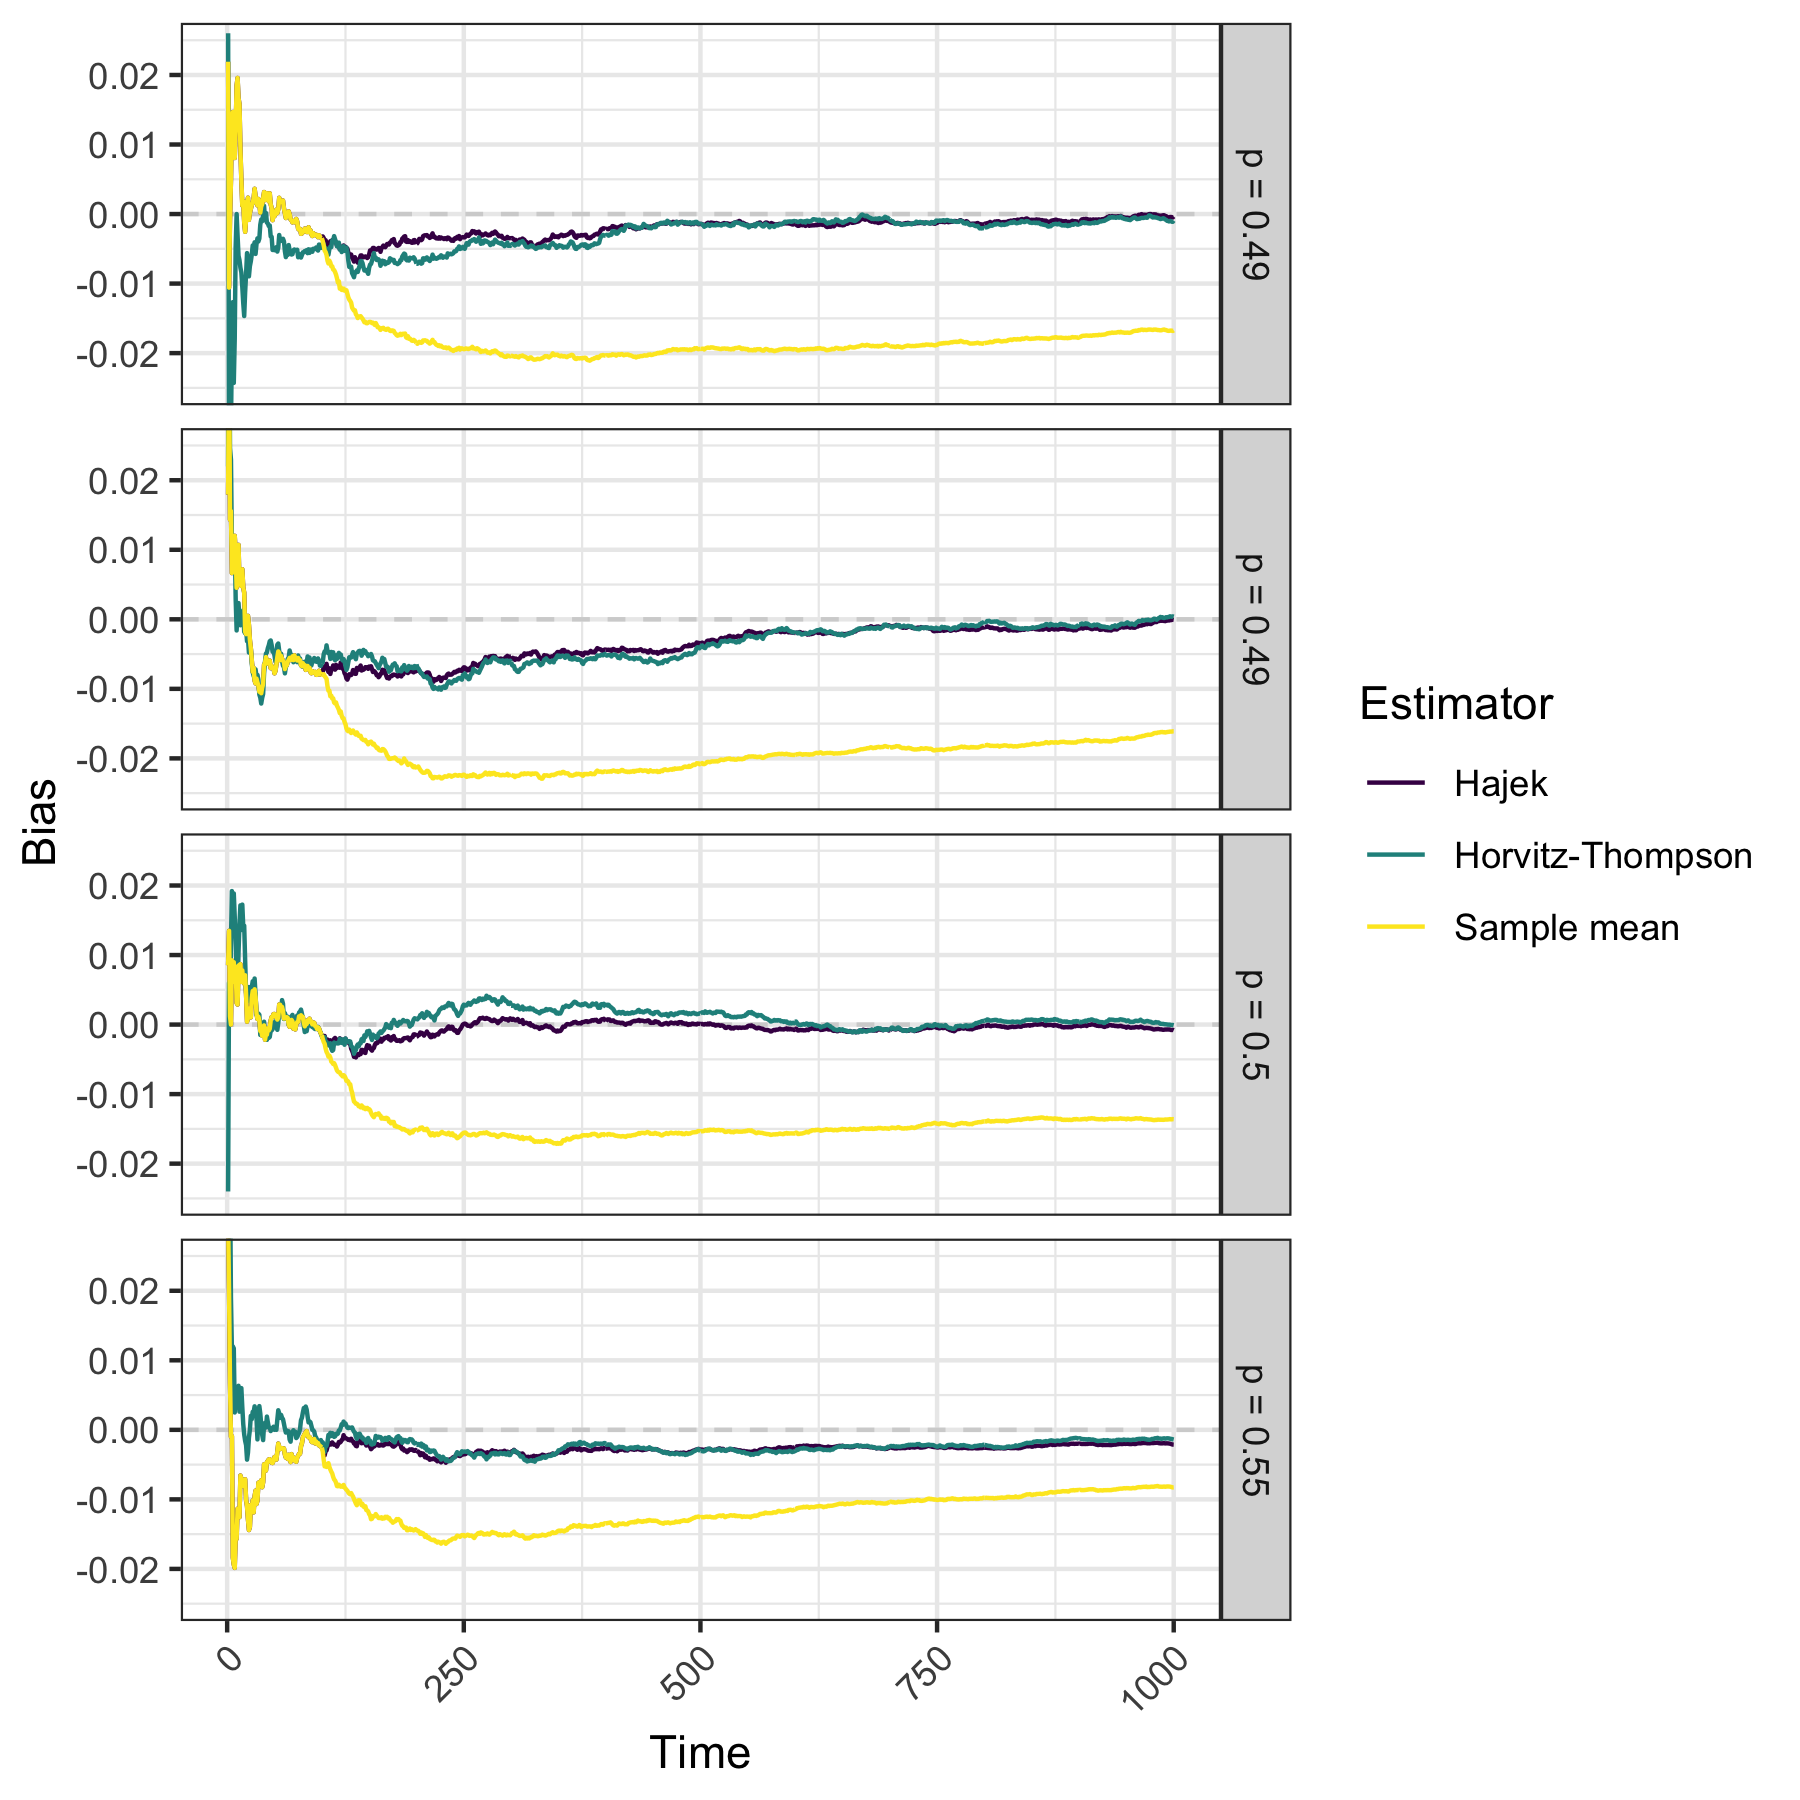
\includegraphics[width = 0.95\textwidth]{../../tables-figures/tt_bias4.png}
   \caption{Top-two Thompson sampling, arm assignment across repetitions. Using four arms and success probabilities 0.49, 0.49, 0.5, and 0.55, this figure shows bias for each arm under different estimators over repeated simulated experiments. }
   \label{fig:ttt_bias}
\end{figure}

\subsection{Evaluation phase}
Following the learning phase, the subsequent 9,000 respondents in each country participate in the evaluation phase. In the evaluation phase, we compare response under the concern-responding chatbot condition to control groups. For group 0, we deliver the survey only. For group 1, we deliver general messaging related to the importance of getting the COVID-19 vaccine when it is made available (see Figure~\ref{fig:psa}). Group 2 receives the concern-responding chatbot condition. 

In the evaluation phase, we assign treatment to all conditions (group 0, 1, and 2) at random. To respondents assigned to group 2, the concern-responding chatbot, we will only deliver the messaging selected for respective concerns during the learning phase. In other words, this design allows us to first learn what the best treatment for each particular concern is (out of the ones we designed/tested) and then evaluate how well these targeted interventions perform compared to a control and static/generic message condition.

With a total of 18,000 respondents in evaluation, divided into three equally sized groups of 6,000 respondents each, we are powered to detect treatment effects of a magnitude of approximately 0.05 standard deviations. 


\section{Analysis}
Analysis will be conducted only on the responses collected during the evaluation phase. In the group 2: concern-responding chatbot, we will use the revised version of the survey script with messaging selected during the learning phase, conditional on reported concern. 

We will compare the three groups, and will report differences between group 1 and group 0, group 2 and group 0, and group 2 and group 1. We test these differences as independent hypotheses. 

\subsection{Main effect estimates}

We will report effects for the response variables combined across countries, and separately for each country:
\begin{itemize}
\item Simple difference in means estimates using heteroskedasticity-consistent (HC2) standard errors \citep{mackinnon1985some}.
\item Treatment effect estimates conditioning on covariates described in the table below, using the Lin estimator \citep{lin2013agnostic}, as implemented in the estimatr R package \citep{blair2021package} using heteroskedasticity-consistent (HC2) standard errors. 
\item Doubly robust estimates, using the known balanced assignment weights and a causal forest model, implemented using the grf package \citep{Tibshirani:2021}. Covariates for adjustment are the same as above. Standard error estimates are produced by the software using the delta method described in section 4 of \cite{athey2019generalized}. 
\end{itemize}

From the follow-up survey, we only report analysis on self-reports of whether respondents have received the vaccine. 

\clearpage


\begin{table}[H]
\begin{adjustbox}{totalheight=.9\textheight-2\baselineskip, max width = \textwidth}
\begin{tabular}{p{0.3\linewidth}p{0.7\linewidth}p{0.25\linewidth}}
\textbf{Covariate}                   & \textbf{Response options} & \textbf{Coded as}                                     \\
\hline
Gender                                              & Male, Female, Nonbinary, Other                                                                                                                                                                                                      & 1 if male, 0 otherwise                                                                         \\
Age                                                 & Integers                                                                                                                                                                                                                            & Continuous, flag if greater than 120                                                           \\
Education                                           & No formal schooling, Informal schooling only, Some primary school, Primary school completed, Some secondary school, Secondary school completed, Post-secondary qualifications, Some university, University completed, Post-graduate & 1:10, flag if missing                                                                          \\
Geography                                           & Urban, Rural                                                                                                                                                                                                                        & 1 if urban, 0 otherwise                                                                        \\
Religion                                            & Christian, Muslim, Other/None                                                                                                                                                                                                       & Indicators                                                                                     \\
Denomination (Christian)                            & Pentecostal, Other                                                                                                                                                                                                                  & Indicator (coded 1 if Pentecostal, 0 otherwise)                                                \\
Religiosity (freq. of attendance)                   & Never, Less than once a month, One to three times per month, Once a week, More than once a week but less than daily, Daily                                                                                                          & 1:6, flag if missing                                                                           \\
Digital Literacy Index                              & {[}Based on the first nine items of the proposed measure in \cite{guessetal2020digital}, see survey instrument for full questions and response options{]}                                                                                         & 0:24                                                                                           \\
Frequency of social media usage (x2)                & {[}See survey instrument for full questions and response options{]}                                                                                                                                                                 & 0:3, flag if missing                                                                           \\
Index of household possessions                      & I/my household owns, Do not own {[}See survey instrument for items{]}                                                                                                                                                               & Continuous, sum of owned items, flag if all missing                                            \\
Job with cash income                                & Yes, No                                                                                                                                                                                                                             & 1 if yes                                                                                       \\
Number of people in household                       & Integers                                                                                                                                                                                                                            & Continuous, flag if missing                                                                    \\
Political affiliation:                              & Governing party v. opposition                                                                                                                                                                                                       & Indicator (coded 1 if associate with or voted for candidate from governing party, 0 otherwise) \\
Health access: hours to hospital                    & Integers                                                                                                                                                                                                                            & Continuous                                                                                     \\
Covid knowledge index                               & True/False                                                                                                                                                                                                                          & Continuous, sum of correct answers                                                             \\
Concern regarding COVID-19                          & Not at all worried, Somewhat worried, Very worried                                                                                                                                                                                  & 1:3, flag if missing                                                                           \\
Perceived government efficacy on COVID-19           & Very poorly, Somewhat poorly, Somewhat well, Very well                                                                                                                                                                              & 1:4, flag if missing                                                                           \\
Strata of pre-treatment response on primary outcome & Indicators for each of the response options in the two vaccine intentions questions                                                                                                                                                 & 2 x 1:4            
\end{tabular} 
\end{adjustbox}
\footnotesize
\ \ \\
\textbf{Note:} Regarding missingness flags, respondents must respond to chatbot questions to advance in the survey, but for contexts they may enter ``skip'' if they do not wish to answer a given question, with the exception of age, which we check is greater than 18. 
\caption{Covariates and response options}
\label{cov_long}
\end{table}

\clearpage

%
%\begin{algorithm} \footnotesize
%    \caption{Batchwise top-two Thompson sampling with probability floors}
%    \label{algg:ttts}
%    \begin{algorithmic}[1] % The number tells where the line numbering should start
%    	\State Set  $\alpha_{k,1} \leftarrow 1, \ \beta_{k,1} \leftarrow 1 \forall k \in \kk ; \aB \leftarrow \y \leftarrow $ empty vector.  
%	\Comment{Initialize priors, assignment vector, and reward vector. }
%    	\For{$i = 1, \dots, N$}
%		\If{$i \in \mathcal{I}_1$}
%			 \State Set $p_{k} \leftarrow \frac{1 }{|\kk| } \ \ \forall k \in \kk $ \Comment{In first batch, set treatment probabilities as uniform.}
%		\ElsIf{$i \in \mathcal{I}_b$ for $b = 2, \dots, B$} 
%			\If{ $i$ is the first observation in $\mathcal{I}_b$} \Comment{At the start of each batch\dots}
%				\For{$k \in \kk$} \Comment{\dots update the distributions.}
%					\State $(\alpha_{k,b}, \beta_{k,b}) \leftarrow (\sum\limits_{i} \mathbbm{1}\{ a_i = k\}\mathbbm{1}\{ y_i = 1\} + 1, \sum\limits_{i}\mathbbm{1} \{ a_i = k\}\mathbbm{1}\{ y_i = 0\})$.
%				\EndFor
%			\EndIf			
%			\For{$k \in \kk$}
%				\State Sample $\hat \theta_k  \sim \textrm{Beta}\left(\alpha_{k,b}, \beta_{k,b} \right)$ \Comment{Sample from posteriors. }
%			 \EndFor
%			\State Set $I_1 \leftarrow \underset{k}{\argmax} \hat\theta_k$; set $I_2 \leftarrow \underset{j}{\argmax} \hat\theta_j, j\neq I_1$. \Comment{Identify top two arms from posterior samples}. 
%			\State Set $p_k \leftarrow \frac{1 }{\delta \times |\kk| } $ for $k \notin \{ I_1, I_2\} $. \Comment{Assign probabilities floors for not top two arms.}
%			\State Set $p_k \leftarrow \frac{1}{2} (1-  \sum\limits_{j \notin \{ I_1, I_2\} } p_j) $ for $k \in \{ I_1, I_2\} $ \Comment{Assign remaining probability to top two arms.}
%		\EndIf
%		\State Assign treatment $a_i$ with probabilities $\p = \{ p_k: k \in \kk \} $; observe rewards $y_i$.
%		\State $\aB \leftarrow [\aB : a_i]$ \Comment{Augment assignment vector.}
%		\State $\y \leftarrow [\y : y_i]$ \Comment{Augment reward vector vector.}
%	\EndFor
%    \end{algorithmic}
%\end{algorithm}

\subsection{Heterogeneity analysis}
We will report conditional average treatment effects for respondents based on the below covariates measured prior to delivery of treatment. 
\begin{itemize}[noitemsep, topsep=0pt]
\item Country (Kenya, Nigeria)
\item Digital literacy (above vs. below median)
\item Age (above vs. below median)
\item Scientific knowledge (above vs. below median)
\item Access to health services (above vs. below median)
\item Gender (binary measurement, female vs. other responses)
\item Political Partisanship (binary measurement, aligned with incumbent political party)
\item Religion (denomination) and religiosity (above vs. below median)
\end{itemize}

Conditional average treatment effects will be reported using the same estimators as under main effects (difference in means, Lin covariate-adjusted estimator, doubly robust estimates using causal forest conditional means model). With three equally sized groups of 6,000 respondents each, we are powered to detect subgroup heterogeneity across equally sized subgroups with effect magnitudes of approximately 0.07 standard deviations. 

\subsection{Attrition}
We collect pre-test responses to the primary outcome of interest, vaccine intentions. This is collected prior to randomization to treatment conditions for all respondents. For respondents who attrit after randomization, we impute post-test responses to the primary outcome as equivalent to the pre-test responses, i.e., as if there is no treatment effect at all. For the secondary outcomes of information seeking and encouragement, we impute zeros, i.e., that respondents did not click through for more information or share posts with peers, which is in line with their actual behavior. 

For sharing behavior, we report both unadjusted, and re-weighted doubly robust estimates, where the weighting accounts for both treatment propensity and missingness propensity, under the assumption that missingness is ignorable conditioning on measured covariates and treatment. 

In the follow-up survey where we elicit vaccination status, we report both unadjusted, and re-weighted doubly robust estimates, where the weighting accounts for both treatment propensity and missingness propensity, under the assumption that missingness is ignorable conditioning on measured covariates, treatment, and primary response.  

\section{Ethical considerations}

This section goes into more detail for some of the design decisions we made as they relate to ethical considerations and concerns. First, while we considered asking individuals to post their vaccine card or SMS confirming their vaccine appointment in the follow up survey we decided against doing so because of privacy reasons. We also didn't want individuals to get into the habit of sharing this information as it may make them more susceptible to scams requesting this information. Second, because we are concerned about the connection between the spread of misinformation about the vaccine and vaccine hesitancy, we wanted to measure respondents' intentions to share both true and false posts as an outcome of the study. We believe the potential benefit to understanding how to reduce sharing of misinformation is greater than the potential risk of showing this information to respondents. However, we also take several measures to mitigate the risk associated with this. Specifically, the false post we show respondents is something that has actually circulated online in both countries and has been debunked. In addition, we do not allow respondents to share this post directly but instead ask for their intention to share and we inform all respondents that this post is untrue. Similarly, we ask a few true/false questions about common misperceptions about COVID and the vaccine during the survey and provide respondents with the true information immediately after they answer these few questions. Finally, we considered including answer options to the concerns about the COVID-19 vaccine question that related to specific rumors (e.g. I don't think the vaccine is safe for pregnant women) but decided against this as we didn't want to emphasize these rumors as possible viewpoints--potentially giving them more credence. The only ``misinformation'' answer option included is ``I don't think COVID-19 is real'' which we felt is less harmful as it's a broad belief, not a specific piece of falsifiable misinformation. 

\clearpage
\bibliography{../fb_chatbot}

\clearpage
\appendix
\section{Power calculations for arm selection}

Scripts for power calculations are posted at \url{https://github.com/UChicago-pol-methods/vaccine-confidence-chatbot/blob/main/code/power_calculations.R}



\end{document}